% Template LaTeX file for DAFx-08 papers % (fold)
%
% To generate the correct references using BibTeX, run
%     latex, bibtex, latex, latex
% modified...
% - from DAFx-00 to DAFx-02 by Florian Keiler, 2002-07-08
% - from DAFx-02 to DAFx-03 by Gianpaolo Evangelista
% - from DAFx-05 to DAFx-06 by Vincent Verfaille, 2006-02-05
% - from DAFx-06 to DAFx-07 by Vincent Verfaille, 2007-01-05
%                          and Sylvain Marchand, 2007-01-31
% - from DAFx-07 to DAFx-08 by Henri Penttinen, 2007-12-12
%                          and Jyri Pakarinen 2008-01-28
%
% Template with hyper-references (links) active after conversion to pdf
% (with the distiller) or if compiled with pdflatex.
%
% 20060205: added package 'hypcap' to correct hyperlinks to figures and tables
%                      use of \papertitle and \paperauthorA, etc for same title in PDF and Metadata
%
% 1) Please compile using latex or pdflatex.
% 2) If using pdflatex, you need your figures in a file format other than eps! e.g. png or jpg is working
% 3) Please use "paperftitle" and "pdfauthor" definitions below


%%%%%%%%%%%%%%%%%%%%%%%%%%%%%%%%%%%%%%%%%%%%%%%%%%%%%%%%%%%%%%%%%%%%%
%%%%%%%%%%%%%%%%%%%%%%%%%%%%%%%%%%%%%%%%%%%%%%%%%%%%%%%%%%%%%%%%%%%%%
%%%%%%%%%%%%%%%%%%%%%%%%%%%%%%%%%%%%%%%%%%%%%%%%%%%%%%%%%%%%%%%%%%%%%
% 
% TTBlue Notes / Paper
% from conversation with Dave over coffee at Pre en Bulle in Albi
% 20 June 2008
% 
% 
% TTBlue is different from existing DSP libraries (such as Perry Cook's STK) in a number of ways:
% * Dynamic environment which itself can be queried for available components (using the TTFactory registry)
% * Dynamic binding, message passing architecture (reflective programming)
% 
% 
% Different from other C++ libraries in that it provides reflective programming techniques.
% Different from other languages with similar features in that it is implemented in C++ with good support for multiple platforms including embedded processor.
%  IEC 61508
%  Isograph
% 
% 
% Allows for:
% * programmatic creation of user interfaces
% * adaptive wrappers for various plug-in architectures (VST, AU, Max/MSP, SuperCollider)
% * dynamic, self-modifying networks of components 
% 
% 
% 
% 
% Try to see what we can learn from:
% * SuperCollider spawning thing for granular synthesis?
%  
% 
% 
% 
% Dynamic re-configuration of the signal networks and control structures means that TTBlue can be run on a web server and the signal chain defined (or re-defined) in real time on a web client using a GUI (such as a web browser or iPhone) or SMS.
% 
% One application of this is an installation or sculptural art work where you could tweak the behavior by sending it SMS messages using a phone.


% I would also like to develop a systematic approach for dealing with interpolation algorithms...
% Some sort of an interpolation library in TTBlue
% For example, this would allow us to apply the cubic interpolation everywhere without re-writing the code


%%%%%%%%%%%%%%%%%%%%%%%%%%%%%%%%%%%%%%%%%%%%%%%%%%%%%%%%%%%%%%%%%%%%%
%%%%%%%%%%%%%%%%%%%%%%%%%%%%%%%%%%%%%%%%%%%%%%%%%%%%%%%%%%%%%%%%%%%%%
%%%%%%%%%%%%%%%%%%%%%%%%%%%%%%%%%%%%%%%%%%%%%%%%%%%%%%%%%%%%%%%%%%%%%




%------------------------------------------------------------------------------------------
%  !  !  !  !  !  !  !  !  !  !  !  ! user defined variables  !  !  !  !  !  !  !  !  !  !  !  !  !  !
% Please use these commands to define title and author of the paper:
\def\papertitle{The Jamoma Multicore Audio Graph Layer}
\def\paperauthorA{Timothy Place?}
\def\paperauthorB{Trond Lossius?}
\def\paperauthorC{Nils Peters?}
\def\paperauthorD{Anyone Else?}


%------------------------------------------------------------------------------------------
\documentclass[twoside,a4paper]{article}
\usepackage{dafx_08}
\usepackage{amsmath,amssymb,amsfonts,amsthm}
\usepackage{subfigure,color}
\usepackage{euscript}
\usepackage[latin1]{inputenc}
\usepackage[T1]{fontenc}
\setcounter{page}{1}
\ninept

\usepackage{times}
% Saves a lot of ouptut space in PDF... after conversion with the distiller
% Delete if you cannot get PS fonts working on your system.

% pdf-tex settings: detect automatically if run by latex or pdflatex
\newif\ifpdf
\ifx\pdfoutput\relax
\else
   \ifcase\pdfoutput
      \pdffalse
   \else
      \pdftrue
\fi

\ifpdf % compiling with pdflatex
  \usepackage[pdftex,
    pdftitle={\papertitle},
    pdfauthor={\paperauthorA, \paperauthorB, \paperauthorC, \paperauthorD},
    colorlinks=false, % links are activated as colror boxes instead of color text
    bookmarksnumbered, % use section numbers with bookmarks
    pdfstartview=XYZ % start with zoom=100% instead of full screen; especially useful if working with a big screen :-)
  ]{hyperref}
  \pdfcompresslevel=9
  \usepackage[pdftex]{graphicx}
  \usepackage[figure,table]{hypcap}
\else % compiling with latex
  \usepackage[dvips]{epsfig,graphicx}
  \usepackage[dvips,
    colorlinks=false, % no color links
    bookmarksnumbered, % use section numbers with bookmarks
    pdfstartview=XYZ % start with zoom=100% instead of full screen
  ]{hyperref}
  % hyperrefs are active in the pdf file after conversion
  \usepackage[figure,table]{hypcap}
\fi

\title{\papertitle}

%-------------SINGLE-AUTHOR HEADER STARTS (uncomment below if your paper has a single author)-----------------------
%\affiliation{\paperauthorA}    % This command replaces \name{The DAFx Crew}
%{\href{http://www.acoustics.hut.fi/dafx08/}{Dept. of Signal Processing and Acoustics,} \\ Helsinki University of Technology, TKK \\ Espoo, Finland\\
%{\tt \href{mailto:dafx-08@acoustics.hut.fi}{dafx-08@acoustics.hut.fi}}}
%-----------------------------------SINGLE-AUTHOR HEADER ENDS------------------------------------------------------

%---------------TWO-AUTHOR HEADER STARTS (uncomment below if your paper has two authors)-----------------------
%\twoaffiliations{\paperauthorA, \sthanks{This work was supported by the XYZ Foundation}}
%{\href{
%http://www.acoustics.hut.fi/dafx08/}{Dept. of Signal Processing and Acoustics,} \\ Helsinki University of Technology, TKK \\ Espoo, Finland\\
%{\tt \href{mailto:dafx-08@acoustics.hut.fi}{dafx-08@acoustics.hut.fi}}
%}
%{\paperauthorB,\sthanks{This guy is a very good fellow}}
%{\href{http://www.acoustics.hut.fi/dafx08/}{Reading Group, Dept.~of Reading Sciences} \\ Univ.~of Universe, Sun \\ {\tt \href{mailto:dafx-08@acoustics.hut.fi}{dafx-08@acoustics.hut.fi}}
%}
%-------------------------------------TWO-AUTHOR HEADER ENDS------------------------------------------------------

%---------------THREE-AUTHOR HEADER STARTS (uncomment below if your paper has three authors)-----------------------
%\threeaffiliations{\paperauthorA, \sthanks{This work was supported by the XYZ Foundation}}
%{\href{
%http://www.acoustics.hut.fi/dafx08/}{Dept. of Signal Processing and Acoustics,} \\ Helsinki University of Technology, TKK \\ Espoo, Finland\\
%{\tt \href{mailto:dafx-08@acoustics.hut.fi}{dafx-08@acoustics.hut.fi}}
%}
%{\paperauthorB,\sthanks{This guy is a very good fellow}}
%{\href{http://www.acoustics.hut.fi/dafx08/}{Reading Group, Dept.~of Reading Sciences} \\ Univ.~of Universe, Sun \\ {\tt \href{mailto:dafx-08@acoustics.hut.fi}{dafx-08@acoustics.hut.fi}}
%}
%{\paperauthorC,\sthanks{She is a member of the Wheel Association}}
%{\href{http://www.acoustics.hut.fi/dafx08/}{Spinning Group, Dept.~of Turning Sciences} \\ Univ.~of Planets, Mars \\ {\tt \href{mailto:dafx-08@acoustics.hut.fi}{dafx-08@acoustics.hut.fi}}
%}
%-------------------------------------THREE-AUTHOR HEADER ENDS------------------------------------------------------

%----------------FOUR-AUTHOR HEADER STARTS (uncomment below if your paper has four authors)-----------------------
\fouraffiliations{
\paperauthorA, \sthanks{This work was supported by BEK and GMEA}}
{\href{http://74objects.com}{74 Objects LLC,} \\ Kansas City, Missouri, USA\\
{\tt \href{mailto:tim@74objects.com}{tim@74objects.com}}
}
{\paperauthorB,\sthanks{This guy is a very good fellow}}
{\href{http://www.acoustics.hut.fi/dafx08/}{Reading Group, Dept.~of Reading Sciences} \\ Univ.~of Universe, Sun \\ {\tt \href{mailto:dafx-08@acoustics.hut.fi}{dafx-08@acoustics.hut.fi}}
}
{\paperauthorC,\sthanks{She is a member of the Wheel Association}}
{\href{http://www.acoustics.hut.fi/dafx08/}{Spinning Group, Dept.~of Turning Sciences} \\ Univ.~of Planets, Mars \\ {\tt \href{mailto:dafx-08@acoustics.hut.fi}{dafx-08@acoustics.hut.fi}}
}
{\paperauthorD,\sthanks{Yes, senior}}
{\href{http://www.acoustics.hut.fi/dafx08/}{Unknown Group, Dept.~of Volatile Sciences} \\ Univ.~of Nowhere, Somewhere \\ {\tt \href{mailto:dafx-08@acoustics.hut.fi}{dafx-08@acoustics.hut.fi}}
}
%-------------------------------------FOUR-AUTHOR HEADER ENDS------------------------------------------------------

% (end)

\begin{document}
% more pdf-tex settings:
\ifpdf % used graphic file format for pdflatex
  \DeclareGraphicsExtensions{.png,.jpg,.pdf}
\else  % used graphic file format for latex
  \DeclareGraphicsExtensions{.eps}
\fi

\maketitle


%%%%%%%%%%%%%%%%%%%%%%%%%%%%%%%%%%%%%%%%%%%%%%%%%%%%%%%%%%%%%%%%%%%%%%%%%%%%%%%%%%%%%%%%%%%


\begin{abstract}

Jamoma Multicore is really cool.

\end{abstract}


%%%%%%%%%%%%%%%%%%%%%%%%%%%%%%%%%%%%%%%%%%%%%%%%%%%%%%%%%%%%%%%%%%%%%%%%%%%%%%%%%%%%%%%%%%%


\section{Introduction} % (fold)
\label{sec:intro}

If you want to be cool, then you need to use Jamoma Multicore too...  We are about to explain why.  

Jamoma Multicore is build upon the Jamoma Foundation and DSP Libraries \cite{Place:2010}.

should mention the license either here or in the abstract.


% TODO: Eric Lyon had the following comment about our DSP paper, which I think could be worked-in here as a way to tie the goals of Multicore into the bigger picture:
%
%	I'm most intrigued by this statement, and would be happy to hear more about it in your paper:
%
%		"Perhaps more important, but more difficult to quantify,
%		we believe we’ve created a context in which code is ‘pleas-
%		ant to work with’."
%
%		This seems to be an increasingly important criterion, especially if (as I believe) we're evolving to a much more porous and flexible continuum across data-flow, scripting, and compiled coding as different entry points for musicians, depending on what they need to do. 
%
%		A few other thoughts - maybe worth writing a bit more on SuperCollider, as it is much more flexible and elegant than Max/MSP/Pd in allowing new pieces of DSP to be eased in and out of a performance (compared to the rigid poly~ structure, on the one hand, or glitches whenever new DSP objects are created on the other). 

% (end)



%%%%%%%%%%%%%%%%%%%%%%%%%%%%%%%%%%%%%%%%%%%%%%%%%%%%%%%%%%%%%%%%%%%%%%%%%%%%%%%%%%%%%%%%%%%

\section{Background} % (fold)

% Audio Units / AUGraph in CoreAudio (pull method for graphs)
% MSP/Pd/etc.

% Multithreading
% Grand Central Dispatch (GCD) is now open source


The Max family includes both MSP\cite{Zicarelli:1998} and PureData\cite{Puckette:1996}.

"The Max paradigm can be described as a way of combining pre-designed building blocks into configurations useful for real-time computer music performance."\cite{Puckette:2002_max_at_17}

This description is more similar to Multicore than to DSP.  In fact, The Max environments also define APIs for creating unit generators and provide libraries of these unit generators (or "pre-designed building blocks").  The environments also define an API for message passing in much the same way that the Jamoma Foundation provides.

Domain-Specific Text-Based Languages are similar to the Max Family except that they create networks of Unit Generators using a text interface.  I don't really want to talk about CSound.  Is that really neccesary?  Can I just mention CSound and SuperCollider together in one sentence?



\subsubsection{SuperCollider} % (fold)

Is there anything particularly pertinent here?\cite{McCartney:1996}

SuperCollider combines the unit generators, the audio engine, and an object-oriented language with semantics similar to C and Smalltalk.  SuperCollider is incredibly powerful because of the language constructs and idioms that manipulate the unit generators.  The API for creating unit generators is similar to many other environments we have reviewed.

% (end)

\subsubsection{ChucK} % (fold)

Probably a bit more here that is pertinent.  Ge Wang might balk at calling ChucK a domain-specific language, but that's what it really is.

``the design of ChucK strives to “hide the mundane aspects of programming, and expose true control”''\cite{wang:2008}.

Unfortunately, ChucK is not suitable for use by Jamoma due to the excessive restrictiveness of the GNU GPL, under which it is licensed.

To it's own admission, execution speed is not the primary priority for ChucK.  As such it does not perform frame-based signal computation but computes at every sample.  This contributes to ChucK's strong timing model, but at the expense of slower number-crunching for audio.

% NOTE: ChucK audio processing is driven by the sink on the graph, using a pull model as we do in Multicore 


% TODO: Do we need to mention something about CMix and RTCMix?
% (end)



\subsubsection{TANGA} % (fold)

TANGA provides and interesting environment because the audio engine is explicitly multi-threaded and thus multi-core capable\cite{Reiter:2007}.  However, it doesn't fit the bill because it is targeted at one context: MPEG-4 scene rendering.  We need something more general.  And it doesn't matter because we are thread-agnostic.

TANGA does provide a message passing interface and a plug-in or extension API.



ZenGarden will need a mention.


\subsection{CLAM} % (fold)

``CLAM stands for C++ Library for Audio and Music and it is a full-fledged software framework for research and application development in the audio and music domain with applicability also to the broader multimedia domain. It offers a conceptual model; algorithms for analyzing, synthesizing and transforming audio signals; and tools for handling audio and music streams and creating cross-platform applications.''

``CLAM, a C++ software framework, that offers a complete development and research platform for the audio and music domain. It offers an abstract model for audio systems and includes a repository of processing algorithms and data types as well as all the necessary tools for audio and control input/output. The frame- work offers tools that enable the exploitation of all these features to easily build cross-platform applications or rapid prototypes for media processing algorithms and systems.'' 

Like Jamoma DSP, it is cross-platform (Mac, Linux, and Windows) and uses automatic integrated building, testing, versioning systems, and generally subscribes to Agile Development practices\footnote{\url{http://en.wikipedia.org/wiki/Agile_software_development}}.  

Full featured, but very complex.  It tries to be a framework, complete with visual editors, for building entire applications.

A key feature of CLAM is it's so-called ``metamodel'', which is a programming layer for creating hierarchical graphs of objects to produce a signal processing chain.  Jamoma DSP does not define the way in which one must produce signal processing topographies.  Instead, the process of creating objects and connecting them are envisioned and implemented orthogonally and the graph is created using a separate framework known as Jamoma Multicore.  Thanks to this decoupling of Jamoma DSP and Jamoma Multicore you aren't ``boxed-in'' to any particular way of creating connections between objects.

Jamoma DSP objects do this as well, via the "calculate" and "process" methods.  Also, like CLAM, all objects provide an interface for working on data and support "metaobject-like facilities such as reflection and serialization".

Well, actually, nothing is synchronous or asynchonous in Jamoma DSP/Foundation.  We are synchronously-agnostic.  Multicore is cable of operating the lower-level DSP in a synchronous matter, as can MSP or Pd or AU etc...

Similar to CLAM, Jamoma Foundation objects have life-cycle state management.  In Jamoma DSP an object can be flagged as valid and/or busy.  CLAM differentiates between "controls" which are attributes that can be changed at any time and "configurations" which require the object to not be busy ("running" in CLAM parlance).  Jamoma DSP does not make this distinction externally: both are simply considered "attributes" and the locking or other requirements are handled internally. 


% TODO: We don't need all this text above, we just need to summarize it.  Something like this:

Many environments such as CLAM \cite{Amatraian:2008} are designed as a monolithic system.  We have taken a more modular approach by creating a series of systems which may work together to provide a complete audio development and research platform.




\subsection{SndObj} % (fold)

The SndObj\cite{Lazzarini:2001} library provides a number of classes much like the STK.  It uses frame-based audio processing routines, as we desire.  One problem is that the frame size (or vector size in SndObj parlance) is an attribute of the object rather than an attribute of the signal being passed to the object.  This may appear to be a subtle difference, but the result is that the process routines cannot adapt to varying vector sizes on-the-fly, such as those produced in contexts such as IRCAM's Gabor \cite{Schnell:2005_Gabor}.



% (end)

%%%%%%%%%%%%%%%%%%%%%%%%%%%%%%%%%%%%%%%%%%%%%%%%%%%%%%%%%%%%%%%%%%%%%%%%%%%%%%%%%%%%%%%%%%%

\section{Design} % (fold)

One example the demonstrates the need for dynamic vectorsizes is the gabor.psola.pat example from FTM. Also granular approaches may benefit (for example, implementing some of the ideas from Curtis Roads' engine).

\subsection{Structure} % (fold)

A graph has many objects.\\
An object has many inlets.\\
An inlet has many inputs.\\
An input has many channels.\\

% (end)

Some important things to keep in mind:

Priorities, how to we control the order of operations?

Matrix mixer/router development, with particular thought about what happens when 5.1 audio is routed to stereo etc.

Signals of varying data rate (for example as proposed by Pulkki), e.g. compressed signals or higher res signals

Signals of steady data rate but varying vector/buffer size (as in FTM/Gabor)

Dynamic number of channels (perhaps useful for FFT and spectral processing?)

Would be ideal if we could have a wrapper for standard MSP external objects as Multicore objects. 
Call the DSP method directly from this wrapper?
Create our own internal DSP chain for it?
start simple as with biquad~, meaning 1 in and 1 out...
it seems like the easiest way out is to just use patcher scripting.



% (end)





%%%%%%%%%%%%%%%%%%%%%%%%%%%%%%%%%%%%%%%%%%%%%%%%%%%%%%%%%%%%%%%%%%%%%%%%%%%%%%%%%%%%%%%%%%%

\section{Implementation} % (fold)

Jamoma Multicore is a layer for wrapping DSP (TTBlue) objects to be used in processing graphs. The implementation of Multicore is not tied to any particular environment, though it is readily adapted to real-time graphical environments. One practical implementation of Jamoma Multicore is for Cycling '74's Max.

The TTMulticoreObject wraps a TTDSP object such that it is possible to 
build a dynamic graph of audio processing units.

It is implemented as a TTObject so that it can receive dynamically bound messages, 
incliding notifications from other objects.


\subsection{Building the Graph} % (fold)

A Multicore graph consists of a collection of objects that are connected in such a way that they are able to perform digital signal processing tasks. Before such processing can occur, the connections of the graph must be established and the graph configured. This happens as a 3 step process:

A 'reset' method is called on all Multicore objects in the graph. This tells all objects to forget any previous connections.

A 'setup' method is called on all Multicore objects in the graph. This causes objects to establish connections to other objects in the graph (i.e. by passing a message to any object directly below themselves).

An 'init' message is sent, initiated by any/all terminal Multicore objects in the graph and traversing up the graph as detailed below.

A terminal object is one that can be used as the final destination and is responsible for driving the entire graph that is connected to it. When this object calls the init method on any objects that are connected to it, they in-turn call the init method on any objects connected to them, etc., until the init method calls have been propagated to all objects in the chain. This init call is responsible for allocating memory for buffers required for the signals, etc.

% (end)


\subsection{Processing the Graph} % (fold)

Processing the DSP Graph

First, a 'preprocess' method is propagated up the chain from the terminal object.

Second, the audio is pulled from the object above it in the chain, again initiated by the terminal object.

% (end)


% (end)



%%%%%%%%%%%%%%%%%%%%%%%%%%%%%%%%%%%%%%%%%%%%%%%%%%%%%%%%%%%%%%%%%%%%%%%%%%%%%%%%%%%%%%%%%%%

\section{Application} % (fold)

\subsection{Max/MSP} % (fold)

Show it working in Max/MSP


\subsubsection{Jamoma Modular} % (fold)

Nils Says:
There is a new modular branch to start working with the multicore 
externals. The name of the branch is "0.6-multicore".

So far, I mainly introduced in≈ and out≈ in a couple of modules. more to come.
*jmod.sur.multi.in
*jmod.sur.multi.out
*jmod.sur.multi.input
*jmod.sur.multi.aux
*jmod.sur.meters
*jmod.sur.output
*jmod.sur.vbap
*jmod.sur.dbap

So you can start to connect your modules and see what's working and 
what's not.
If you are curious, just check out this branch and try it.
in the git repository, go to Modules/Modular and do a

git checkout 0.6-multicore
% (end)
% (end)


\subsection{Ruby} % (fold)

Here is what a simple \texttt{irb} session should look like:

\begin{lstlisting}
	require 'TTRuby'
 	dac = TTRuby.new("multicore", "output")
 	osc = TTRuby.new("multicore", "wavetable")

	dac.connect(osc)
	dac.start()
	
	osc.set("frequency", 220.0)
\end{lstlisting}



% (end)

% (end)


%%%%%%%%%%%%%%%%%%%%%%%%%%%%%%%%%%%%%%%%%%%%%%%%%%%%%%%%%%%%%%%%%%%%%%%%%%%%%%%%%%%%%%%%%%%

\section{Discussion and Future Work}

\subsection{Multithreading} % (fold)

Multithreading is a big deal.  

- Integrated Analysis and Benchmarking -- perhaps reference the upchuck operator in ChucK?
   -- This integrated analysis and benchmarking could also provide the basis by which an audio graph such as Jamoma Multicore is able to evaluate how to optimize the processes in the graph to make intelligent decisions on how to distribute the processing among threads or processors.

% (End)

\subsection{Implicit Patching} % (fold)

Marsyas is a software framework for building efficient complex audio processing systems and applications \cite{Tzanetakis:2008}. "Audio processing systems are defined hierarchically through composition using implicit patching. Both the specification of the processing network and the control of it while data is flowing through can be performed at runtime without requiring recompilation."

"It is based on a dataflow model of computa- tion in which any audio processing system is represented as a large network of interconnected basic audio process- ing units."  Just like Max/MSP, Pd, Chuck, etc.

One difference to Max/MSP and Pd is that the signal network can be reconfigured dynamically without requiring a 'recompile' of the signal chain.  This is addressed through Jamoma Multicore -- Jamoma DSP is low level and is agnostic about how objects are combined into a network or topology.

However, objects can be recombined and structured at runtime, offering the same kind of flexibility and "expressive power".

\subsubsection{Implicit Patching}

One thing that makes Marsyas special is its notion of "Implicit Patching".  In this paradigm unit generators are added to a collection and their interaction with the signal processing graph is determined according to a pattern such as 'series', 'fanout', etc. \cite{Bray:2005}.

Currently Jamoma DSP (and Multicore) operate solely through an 'explicit' patching paradigm similar to most other frameworks.  "In explicit patching the user would first create the modules and then connect them by explicit patching statements."  Due to the flexibility of the dynamically bound objects, however, it is quite easy to see how the implementation of pattern-based collections might be defined.

% (end)



%%%%%%%%%%%%%%%%%%%%%%%%%%%%%%%%%%%%%%%%%%%%%%%%%%%%%%%%%%%%%%%%%%%%%%%%%%%%%%%%%%%%%%%%%%%

\section{DAFx Template Stuff}

\subsection{Figures}
\label{ssec:figures}
All figures should be centered on the column (or page, if the figure spans both columns).
Figure captions (in italic) should follow each figure and have the format given in Figure \ref{fft_plot}.
\begin{figure}[ht]
\centerline{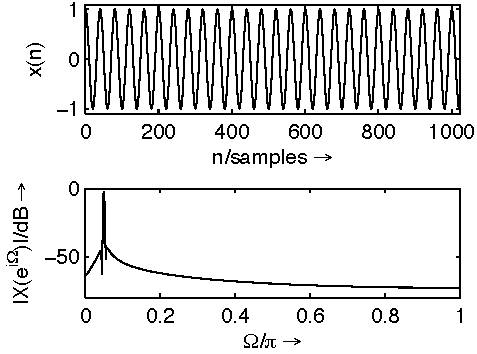
\includegraphics[scale=0.8]{fft_plot2}}
\caption{\label{fft_plot}{\it Sinusoid in time and frequency domain.}}
\end{figure}
Vectorial figures are preferred. For example when using
\texttt{Matlab}, export using either Postscript or PDF format. Also,
in order to provide a better readability, figure text font size
should be at list identical to footnote font size. To do so using
\texttt{Matlab}, use the \texttt{subplot} command before plotting.
If bitmap figures are used, please make sure that the resolution is
enough for print quality. Fig. \ref{ftt_plot2} illustrates an
example of a figure spanning two columns.
\begin{figure*}[ht]
\centerline{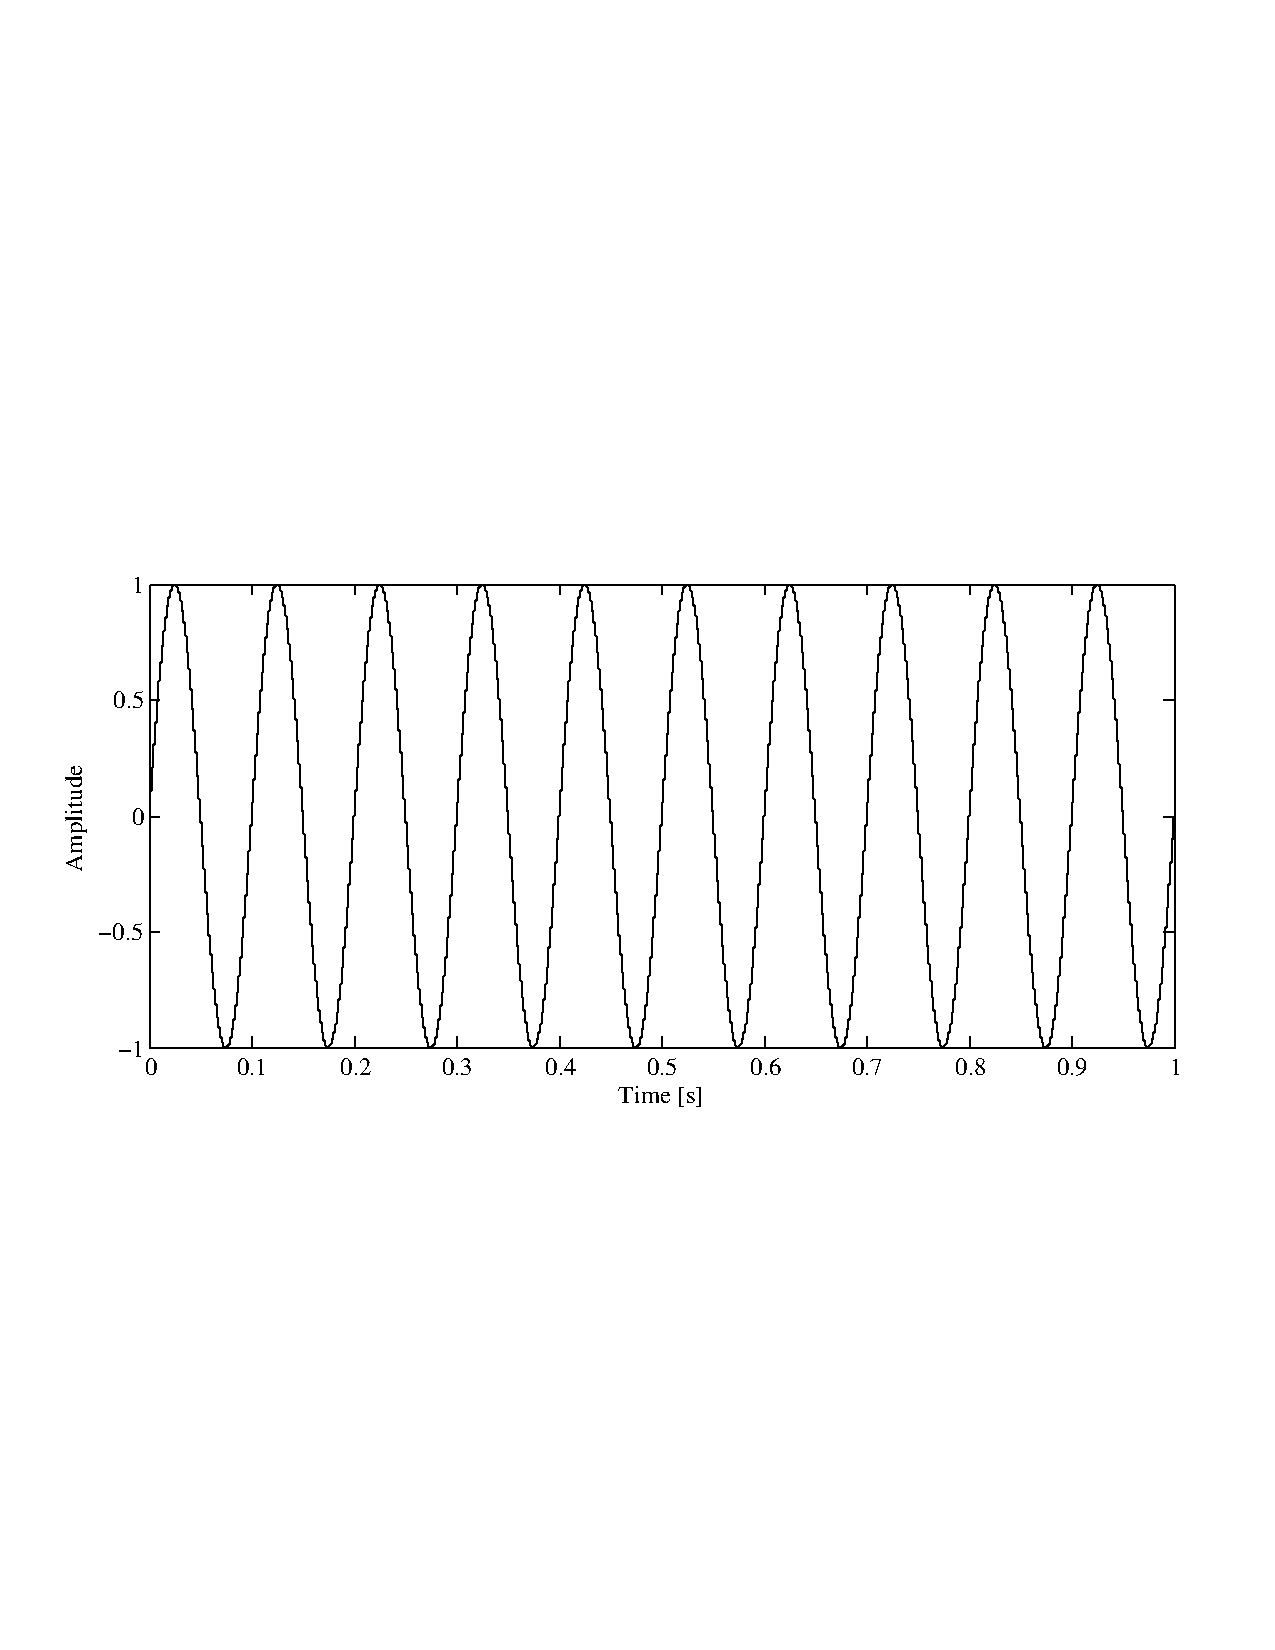
\includegraphics[width=5in,bb= 3 257 607 534]{TwoColumnSine2}} % The bounding box is set manually in this example. Useful for some .pdf figures.
\caption{\label{ftt_plot2}{\it A figure spanning two columns, as mentioned in Sec. \ref{ssec:figures}. }}
\end{figure*} % [width=5in,bb= 36 253 574 500]



%%%%%%%%%%%%%%%%%%%%%%%%%%%%%%%%%%%%%%%%%%%%%%%%%%%%%%%%%%%%%%%%%%%%%%%%%%%%%%%%%%%%%%%%%%%

\section{Conclusions}
We rock.


%%%%%%%%%%%%%%%%%%%%%%%%%%%%%%%%%%%%%%%%%%%%%%%%%%%%%%%%%%%%%%%%%%%%%%%%%%%%%%%%%%%%%%%%%%%

\section{Acknowledgments}
Thanks!


%%%%%%%%%%%%%%%%%%%%%%%%%%%%%%%%%%%%%%%%%%%%%%%%%%%%%%%%%%%%%%%%%%%%%%%%%%%%%%%%%%%%%%%%%%%

\bibliographystyle{IEEEbib}
\bibliography{../../Shared/bibtex/Jamoma} % requires file template.bib

\end{document}
